\section{Apresentação e Discussão dos Resultados}
\label{sec:resultados}

\subsection{Verificação do simulador}
\label{sec:verificacao}

Antes de ser aplicado a 2030, o simulador foi comparado com o balanço observado de 2022 a 2026. A importação observada é calculada com os cortes somados à geração, para ter o mesmo conceito da simulada. No primeiro teste, o simulador recebe o clima, a hidrologia e os níveis observados de cada ano, e usa os modelos finais. No segundo, os modelos são treinados sem o ano testado, e os resíduos desse ano também são excluídos (Tabela~\ref{tab:verificacao}).

\begin{table}[H]
\centering
\caption{Importação anual observada e simulada com os níveis observados de cada ano (TWh). Em 2026, janeiro a outubro, nas horas em que o balanço do ONS fecha.}
\label{tab:verificacao}
\footnotesize
\renewcommand{\arraystretch}{1.15}
\begin{tabular}{@{}lrrr@{}}
\toprule
Ano & Observada & Simulada, modelos finais (erro) & Simulada, ano fora do treino (erro) \\
\midrule
\LinhasVerificacao
\bottomrule
\end{tabular}
\end{table}

Com os modelos finais, o erro vai de \ErroRetroMin\% a \ErroRetroMax\%. Fora da amostra, o simulador subestima a importação em todos os anos, de \ErroForaMenor\% a \ErroForaMaior\%, com os maiores erros em 2025 e 2026. Para localizar a origem do erro, as formas simuladas, isto é, a variação de cada série ao longo do ano em torno da sua média, foram trocadas pelas observadas, e a regra hidráulica foi mantida. Com isso, o erro de 2025 cai para menos de 1\%, e o de 2026, para \ErroFormasMin\%. A maior parte do erro desses dois anos vem, portanto, das formas. Nenhuma das séries o explica sozinha. Os desvios de 2025 e 2026 em relação aos modelos diferem dos de outros anos, dos quais vêm os resíduos sorteados, e por isso o sorteio os reproduz apenas em parte.

Para 2026 há um segundo backtest, com os níveis do cenário de 2026 no lugar dos observados (Figura~\ref{fig:backtest}). Com clima e hidrologia sorteados (A), a importação observada de \ObsVinteSeis~TWh fica no percentil \PercVinteSeis{} da distribuição (P5--P95 de \AMin{} a \AMax~TWh). Essa comparação não é uma previsão, pois os modelos finais usam dados até outubro de 2026. Com clima e hidrologia observados e modelos treinados até 2025 (B), o simulador obtém \BVinteSeis~TWh (\ErroBVinteSeis\%). A margem horária simulada tem correlação de \CorrBVinteSeis{} com a observada e o mesmo sinal em \SinalBVinteSeis\% das horas. 

O erro é menor do que o da Tabela~\ref{tab:verificacao} porque, neste teste, as séries simuladas não são ajustadas às médias observadas. A geração eólica simulada fica 3\% abaixo da observada (com os cortes somados), e a carga, 1\% acima da que fecha o balanço do ONS. As duas diferenças aumentam a importação simulada e compensam parte da subestimação.

\begin{figure}[H]
\centering
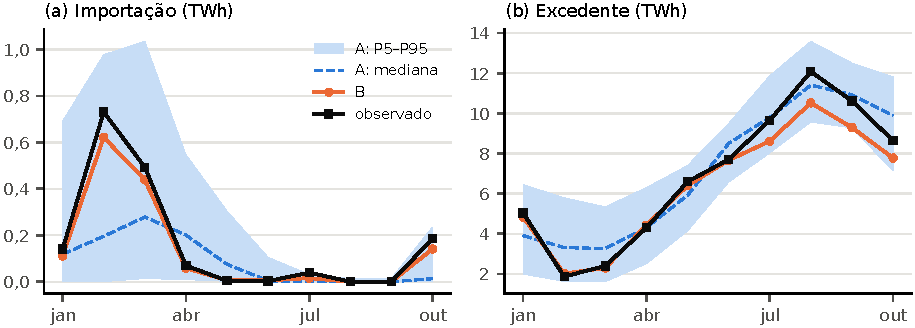
\includegraphics{fig_backtest}
\caption{Importação e excedente mensais de 2026, observados e simulados com os níveis do cenário de 2026. A: clima e hidrologia sorteados. B: clima e hidrologia observados.}
\label{fig:backtest}
\end{figure}

Esses testes indicam que o nível da importação de 2030 tende a estar subestimado. O nível depende também das hipóteses, sobretudo do despacho hidráulico, do nível da carga, da expansão eólica e da data de entrada dos data centers.

\subsection{Importação e excedente em 2030}
\label{sec:importacao2030}

A Tabela~\ref{tab:resultados} resume os resultados. Sem novos data centers e com a expansão eólica base, o Nordeste precisaria importar em média \ImpSem~TWh em 2030, em \HorasSem{} horas do ano. No cenário central, a importação média é de \ImpCen~TWh, em \HorasCen{} horas (\PctHorasCen\% do ano). Um simulador determinístico, que usa os perfis observados de 2022 a 2025 no lugar dos sintéticos, chega a valores próximos: \DetSem~TWh sem data centers e \DetCen~TWh no cenário central. A região continua exportadora em todos os cenários: o excedente médio cai de \ExcSem{} para \ExcCen~TWh no cenário central, e a parcela acima do limite de exportação de 21~GW cai de \ExcLimSem{} para \ExcLimCen~TWh.

\begin{table}[H]
\centering
\caption{Resultados para 2030: média dos sorteios, com P5--P95 entre colchetes. Horas e excedente referem-se à eólica base.}
\label{tab:resultados}
\footnotesize
\renewcommand{\arraystretch}{1.15}
\setlength{\tabcolsep}{5pt}
\begin{tabular}{@{}lrlrrrr@{}}
\toprule
 & & \multicolumn{3}{c}{Importação (TWh)} & & \\
\cmidrule(lr){3-5}
Data centers & MWmed & Eólica base & Eólica baixa & Eólica alta & Horas & Excedente (TWh) \\
\midrule
\LinhasResultados
\bottomrule
\end{tabular}
\end{table}

A importação varia muito de um ano para outro. No cenário central, os percentis 5 e 95 são \ImpCenPCinco{} e \ImpCenPNoventa~TWh, e as distribuições dos cenários se sobrepõem (Figura~\ref{fig:distribuicao}a): a mediana do cenário central (\ImpCenMed~TWh) é menor que o P95 do caso sem data centers (\ImpSemPNoventa~TWh). A maior parte dessa variação vem do clima (Figura~\ref{fig:anos}a). A média do cenário central por ano meteorológico vai de \ImpAnoMin~TWh, com o clima de 2012, a cerca de \ImpAnoMax~TWh, com o de 2009 ou 2020. Na decomposição da variância da importação anual entre os \NSorteios{} sorteios do cenário central, o ano meteorológico responde por \VarClima\%, o ano hidrológico por \VarHidro\% e o restante, que reúne os resíduos e a interação entre os dois anos, por \VarRes\%. O IC95 da média, que considera o número limitado de anos, é de \IcCenMin{} a \IcCenMax~TWh no cenário central e de \IcSemMin{} a \IcSemMax~TWh sem data centers.

\begin{figure}[htb]
\centering
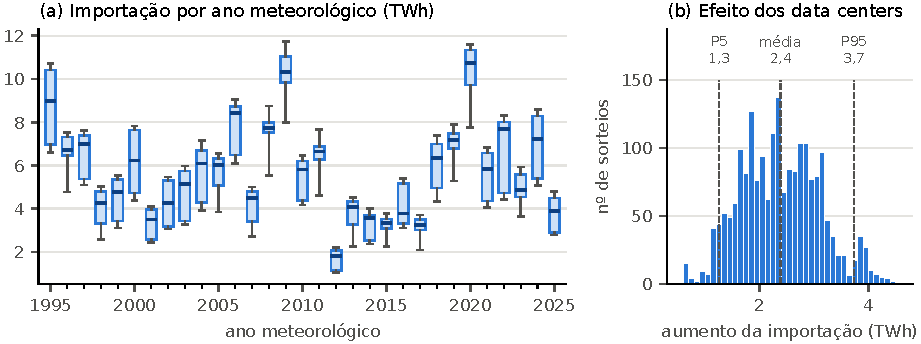
\includegraphics{fig_anos_efeito}
\caption{Cenário central com eólica base: (a) importação anual dos sorteios de cada ano meteorológico, com caixa de P25 a P75, traço na mediana e hastes de P5 a P95; (b) aumento da importação causado pelos data centers em cada um dos \NSorteios{} sorteios, em relação ao caso sem data centers.}
\label{fig:anos}
\end{figure}

\begin{figure}[H]
\centering
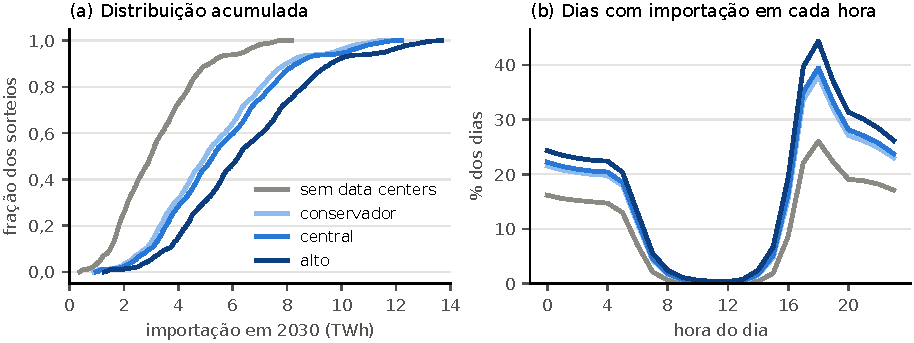
\includegraphics{fig_distribuicao}
\caption{Resultados de 2030 com eólica base: (a) distribuição acumulada da importação anual; (b) percentual de dias com importação em cada hora.}
\label{fig:distribuicao}
\end{figure}

A importação concentra-se no fim da tarde e à noite (Figura~\ref{fig:distribuicao}b). Às 18~horas, quando a solar já cessou e a eólica ainda não subiu, há importação em \PctDezoitoCen\% dos dias no cenário central, contra \PctDezoitoSem\% sem data centers. De madrugada o percentual fica próximo de \PctMadrugada\%, e entre 9 e 13~horas é quase nulo devido ao excedente característico das horas de maior irradiância solar.

\subsection{Efeito dos data centers}
\label{sec:efeito}

Em resumo, no cenário central, os data centers aumentam a importação em \EfCen~TWh por ano (P5--P95 de \EfCenMin{} a \EfCenMax, Figura~\ref{fig:anos}b) e em \EfHoras{} horas. Essa faixa é cerca de três vezes mais estreita que a do nível da importação, porque os dois cenários são comparados no mesmo sorteio, com o mesmo clima. O sinal é positivo por construção, pois a mesma carga adicional é somada a cada sorteio e aumenta a demanda do sistema. No entanto, o que interessa é o aspecto temporal: o aumento de importação equivale a \EfPct\% da energia consumida pelos data centers. Os outros \Absorcao\% são atendidos por geração que, sem eles, seriam horas de excedente. O efeito é de \EfBaixa~TWh com eólica baixa e de \EfAlta~TWh com eólica alta, e o IC95 do valor médio, com eólica base, é de \IcEfMin{} a \IcEfMax~TWh. Não se pode concluir que esse consumo de datacenters evite cortes na mesma proporção em que é atendido pelas horas de excedentes, afinal, parte dos cortes decorre de restrições da rede não representadas. No entanto, o insight importante extraído foi: o papel de aliviar a rede elétrica da sobreoferta de fontes renováveis.

\subsection{Compensação eólica}
\label{sec:compensacao}

Para gerar em um ano a energia consumida pelos data centers do cenário central são necessários \CompEnergia~GW de eólica além da base. Com essa capacidade, a importação média ainda seria de \ImpComEnergia~TWh, acima dos \ImpSem~TWh do caso sem data centers (Figura~\ref{fig:compensacao}). Para voltar a esse nível são necessários \CompImp~GW (P5--P95 de \CompImpMin{} a \CompImpMax), ou \CompRazao{} vezes mais. Para igualar o número de horas com importação, o valor é de \CompHoras~GW. Nos demais cenários, a razão entre os dois primeiros critérios fica entre \RazaoMin{} e \RazaoMax{} e aumenta com a frota eólica.

\begin{figure}[H]
\centering
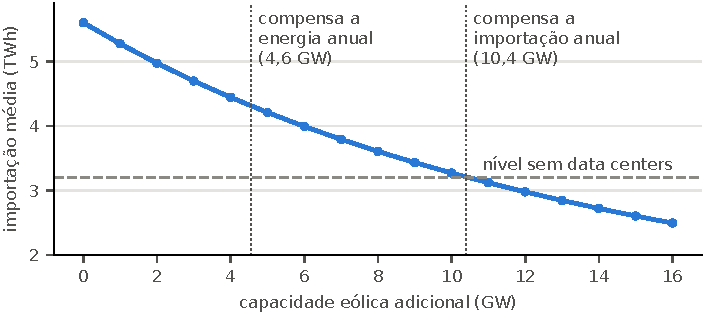
\includegraphics{fig_compensacao}
\caption{Importação média em 2030 no cenário central em função da capacidade eólica adicional (300 sorteios).}
\label{fig:compensacao}
\end{figure}

A diferença conceitual entre essas métricas decorre do perfil da geração. As horas de importação que restam são as de vento fraco, e nelas cada GW adicional gera pouco. Dada a convexidade do gráfico, nota-se que impacto marginal do aumento de geração decresce, pois este é acompanhado de uma redução de horas de importação, para as quais ele contribui no total anual. O cálculo supõe que as novas usinas têm o mesmo perfil horário da frota atual. Uma expansão em locais com regime de vento complementar, ou o armazenamento de energia, mudaria esses valores, mas essas alternativas não foram avaliadas.

\subsection{Sensibilidades}
\label{sec:sensibilidades}

A Figura~\ref{fig:sensibilidades} mostra quanto a importação do cenário central muda quando uma hipótese é alterada. As mais influentes são o despacho hidráulico, o nível da carga, a expansão eólica e a data de entrada dos data centers.

\begin{figure}[H]
\centering
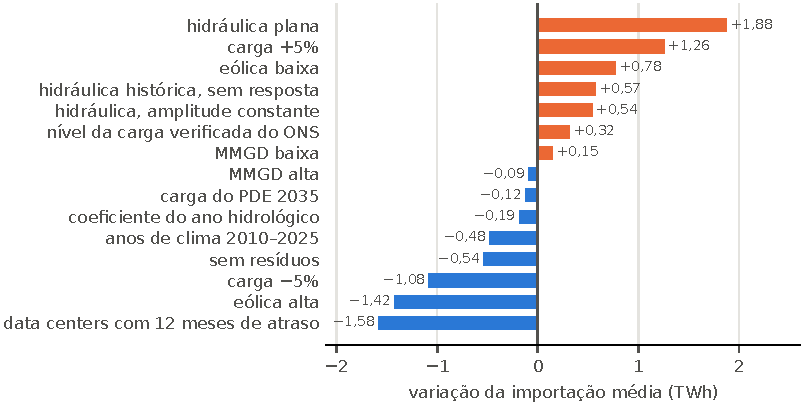
\includegraphics{fig_sensibilidades}
\caption{Variação da importação média do cenário central, com eólica base, em relação à referência (500 sorteios comuns).}
\label{fig:sensibilidades}
\end{figure}

\subsection{Discussão}
\label{sec:discussao}

A variação entre anos encontrada aqui concorda com \textcite{bloomfield2016}, que consideram insuficientes menos de dez anos de dados para o planejamento. A reanálise atende a esse requisito para o vento e a irradiância, mas os quatro anos hidrológicos não. O sorteio também trata o ano meteorológico e o hidrológico como independentes.

\textcite{staffell2016} representam a mudança da frota ao simular cada parque. Aqui, com uma única função para a região, foi preciso treinar em dados recentes, porque as usinas novas geram mais com o mesmo vento. O CF potencial depende da energia cortada apurada pelo ONS, cuja geração de referência mudou ao longo do período, e parte do aumento observado pode vir dessa mudança. A separação entre avaliação \textit{ex ante} e \textit{ex post}, usada por \textcite{hyndman2010}, ajudou a localizar o erro: em 2026, a importação observada é compatível com a distribuição sorteada, e foi o teste com o clima conhecido que revelou a subestimação.

Os picos de importação devem ser lidos com cautela. A média do pico anual é de \PicoSem~GW sem data centers e de \PicoCen~GW no cenário central, acima do maior fluxo de importação registrado de 2022 a 2025 (\FluxoMax~GW). A térmica segue o despacho histórico e não reage à falta de geração, e o estudo não encontrou um limite de importação documentado. Os valores indicam a necessidade calculada se nada mais respondesse e não representam risco de falta de suprimento. Por fim, a projeção oficial de data centers quase triplicou entre a versão original do PLAN e a sua segunda revisão, de modo que os cenários devem ser atualizados a cada nova publicação.
